\chapter{Introducción}

En la actualidad las redes de datos están creciendo en complejidad. Basta mirar el incremento en la cantidad de aplicaciones web que ofrecen contenido multimedia, para determinar que no solo crece el volumen de los datos, sino que además se requiere una mayor velocidad y confiabilidad en la transmisión. 

También es notoria la consolidación de múltiples servicios sobre redes Ethernet, tales como comunicación de voz, vídeo en estándar y alta definición, videoconferencias, transacciones en tiempo real, etc.

En este contexto puede verse como es necesaria la optimización en el procesamiento de los paquetes de datos. Esto debe darse bajo la premisa de que no alcanza con proveer soluciones rápidas, sino que también se debe dotar a las mismas de un buen grado de flexibilidad y escalabilidad que permitan sostener el ritmo actual de crecimiento.



\section{Contexto}
\begin{comment}
\subsection{Evolución en los dispositivos de enrutamiento}

En un principio los enrutadores contaban con un bus central compartido, un CPU, memoria y los puertos de entrada y salida. Cada paquete entrante era transferido al CPU por medio del bus compartido. La decisión de reenvío se llevaba a cabo allí y luego el paquete atravesaba nuevamente dicho bus hacia el puerto de salida. La performance de estos dispositivos estaba limitada principalmente por 2 factores: la capacidad de procesamiento de la CPU central (debido a que la búsqueda en la tabla de ruteo es una tarea que consume una alta cantidad de tiempo) y el hecho de que cada paquete tenía que atravesar 2 veces el bus compartido.

Para hacer frente al primer factor algunos fabricantes de enrutadores introdujeron paralelismo mediante múltiples CPU. Cada una de ellas manipulaba un porción del tráfico entrante. Pero cada paquete tenía todavía que atravesar el bus compartido 2 veces. 

Más adelante el diseño de la arquitectura de enrutadores avanzó un paso más. Una memoria caché de ruteo y capacidad de procesamiento fueron añadidos a cada puerto y las decisiones de reenvío se hacían localmente. De esta manera, cada paquete atraviesa el bus compartido solamente una vez desde el puerto de entrada hacia el puerto de salida. Aunque cada puerto contaba con capacidad de procesamiento, todas las funciones de control todavía se manejaban por el procesador central.

Aunque con el tiempo la performance de los distintos CPU han crecido, este crecimiento no ha podido mantener el ritmo del incremento en la capacidad de los enlaces. Es en este contexto donde se ve claramente que hoy por hoy uno de los mayores cuellos de botella en los enrutadores troncales es el cómputo del prefijo más largo para cada paquete. Los protocolos de hoy en día requieren hacer selección de rutas en base no sólo a un campo sino a varios (tales como el número de protocolo, dirección de origen, puerto de destino, etc). El número de accesos a memoria y la velocidad de ésta determinan la rapidez de un algoritmo de búsqueda de ruta (route lookup algorithm).

\end{comment}

%\subsection{Requerimiento de procesamiento en redes}
%\subsubsection{Características del tráfico}

En lo que respecta a las tecnologías de red, las nuevas tendencias se canalizan hacia la agregación de paquetes en flujos. Dos ejemplos los constituyen conmutación multi-protocolo mediante etiquetas (\textit{Multiprotocol Label Switching}, MPLS) y redes virtuales  de área local (\textit{Virtual LAN}, VLANs). MPLS es un mecanismo en redes de telecomunicaciones de alta performance que transporta datos de nodo a nodo basado en etiquetas en lugar de direcciones de red, con el fin de evitar búsquedas complejas en una tabla de ruteo. Dichas etiquetas se aplican en el inicio de la transmisión e identifican enlaces virtuales entre nodos. También es capaz de encapsular paquetes de varios protocolos de red.

\begin{figure}[h]
  \centering
	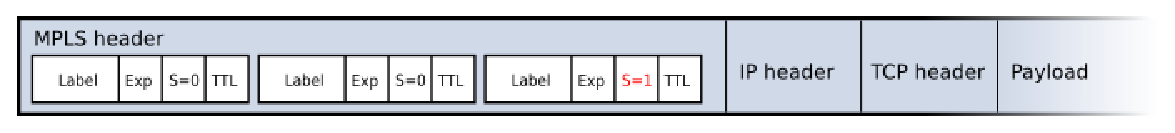
\includegraphics[width=0.99\textwidth]{1-introduccion/graf/MPLS_packet.eps}
  \caption{Encabezado MPLS}
  \label{fig:flow}
\end{figure}
Las VLANs son redes virtuales, lógicamente independientes, que están conectadas a un mismo conmutador físico. Su funcionamiento se basa en un etiquetado dentro de las tramas de enlace de datos. El estándar IEEE 802.1Q es el que domina el mundo de las VLANs.


\begin{figure}[h]
  \centering
	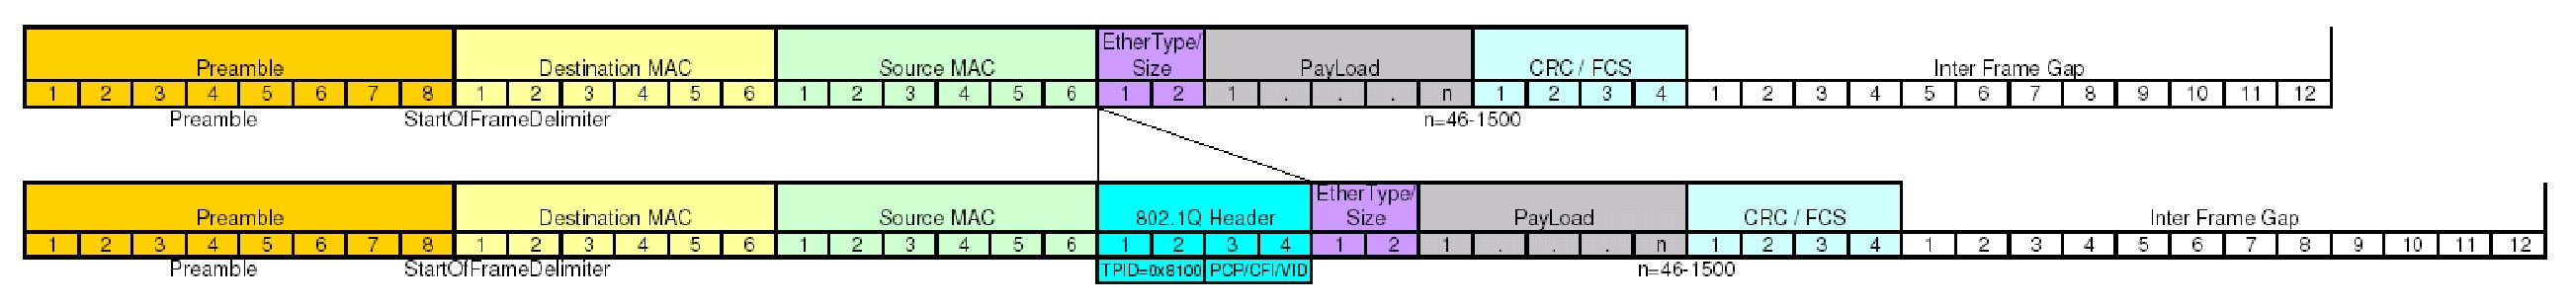
\includegraphics[width=1.1\textwidth]{1-introduccion/graf/TCPIP_802.1Q.eps}
  \caption{Encabezado IEEE 802.1Q en una trama de enlace de datos}
  \label{fig:virt}
\end{figure}


%\subsection{Lógica reconfigurable como respuesta}

En cuanto al hardware necesario para hacer frente a esta brecha entre la necesidad de procesar el flujo creciente de datos de la red y la capacidad de hacerlo, se busca contar con soluciones que permitan generar respuestas específicas de manera flexible, en el menor tiempo y con el mejor rendimiento posible. Las tecnologías que en la actualidad son usadas para implementar soluciones a estos problemas, son tres:

\emph{Los Circuitos Integrados de Propósito Específico (\textit{Application-Specific Integrated Circuit}, ASIC), están formados por cientos de bloques especializados trabajando en paralelo. Aunque cuentan con un muy buen desempeño, tienen un alto costo inicial y el tiempo para desarrollarlos es grande.}

\emph{Los Procesadores de Red (Network Processors, NPs), específicos para este tipo de problemas, ya que cuentan con múltiples elementos de procesamiento, buena performance para ciertas tareas, aunque tienen dificultades de portabilidad debido a que sus interfaces son propietarias en casi todos los casos.}
\begin{figure}[h]
  \centering
      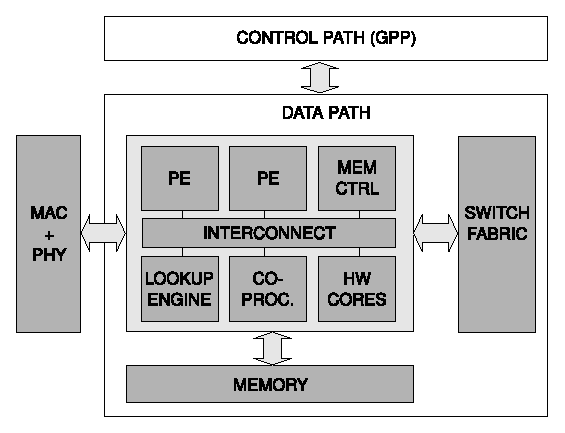
\includegraphics[width=0.5\textwidth]{1-introduccion/graf/NP_based.eps}
  \caption{Solución basada en NP}
  \label{fig:diseno}
\end{figure}
\newpage

\emph{Los Procesadores de Propósito General (General Purpose Processors,GPPs), utilizan la arquitectura propia de la PC y la adaptan al procesamiento de red mediante un software especializado. Aunque esta solución es muy popular por su flexibilidad y su bajo costo, las transacciones con memoria RAM mediante un bus compartido y la naturaleza secuencial de los GPPs son factores limitantes a tener en cuenta. }
 \begin{figure}[h]
  \centering
      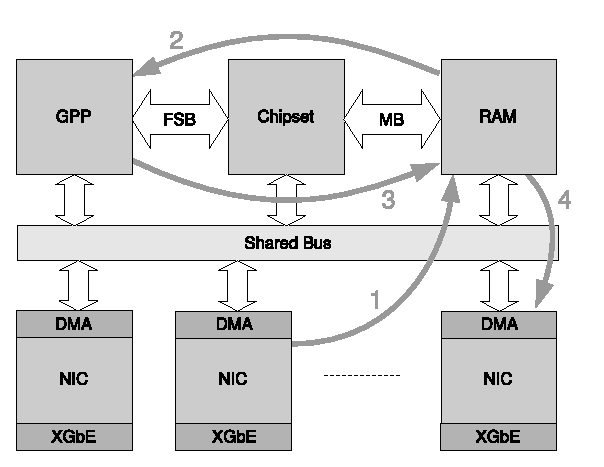
\includegraphics[width=0.5\textwidth]{1-introduccion/graf/GPP_based.eps}
  \caption{Solución basada en GPP}
  \label{fig:diseno}
\end{figure}

Las tecnologías actuales, por las razones anteriormente mencionadas, están alcanzando su límite y es necesario encontrar tecnologías que las reemplacen o que cubran sus falencias, para poder satisfacer los requerimientos actuales de las redes. 

Los FPGAs (Field-Programmable Gate Array) son dispositivos de lógica reconfigurable que es posible programar, una o varias veces, usando un lenguaje de descripción de hardware(\textit{Hardware Description Language}, HDL). Las FPGAs se utilizan en aplicaciones similares a los ASICs; sin embargo son más lentas, tienen un mayor consumo de potencia y no pueden abarcar sistemas tan complejos como los ASICs. A pesar de esto, tienen un flujo de diseño flexible, sus costes de desarrollo y adquisición son mucho menores para pequeñas cantidades de dispositivos y el tiempo de desarrollo es también menor.

%\subsubsection{FPGA como plataforma para SoC}

Los Sistemas en un Chip (\textit{System on Chip}, SoC) son circuitos integrados que contienen todo, o la mayoría, de los módulos que corresponden a un sistema informático o electrónico en un solo componente. Son usados especialmente en el área de sistemas embebidos. Los microcontroladores son técnicamente SoC, pero se considera que los SoC tienen procesadores mas potentes y pueden correr aplicaciones mas complejas, para lo cual necesitan mayor cantidad de memoria que suele estar disponible como chips externos. 

Gracias a la disponibilidad en la ultima década de Soft-Core CPUs y otros Soft IP, se ha producido un punto de inflección en el uso de FPGAs como plataforma para SoC. Como resultado de la combinacion de logros técnicos y fuerzas de mercado, varios fabricantes como Altera, Cypress Semiconductor, Intel y Xilinx anunciaron la comercialización de FPGA con facilidades para el desarrollo de SoC.
Estos avances que simplifican el desarrollo de SoC, la flexibilidad en el flujo de diseño y el prototipado rápido son las condiciones que posicionan a las FPGAs como la herramienta indicada para atacar un problema tan complejo como la clasificación de paquetes. 

 \begin{figure}[h]
  \centering
	 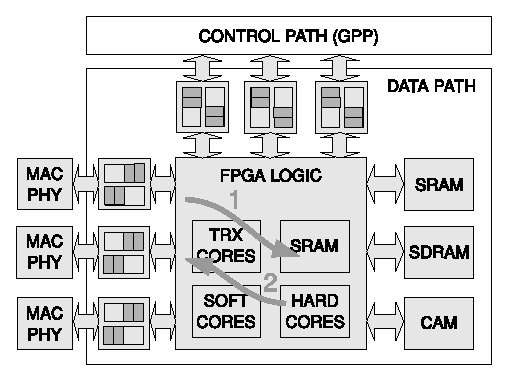
\includegraphics[width=0.5\textwidth]{1-introduccion/graf/FPGA_based.eps}
  \caption{Solución basada en FPGA}
  \label{fig:diseno}
\end{figure}

     




\section{Problema Marco}
\begin{comment}
\subsubsection{Datagrama IP}

\begin{figure}[h]
  \centering
	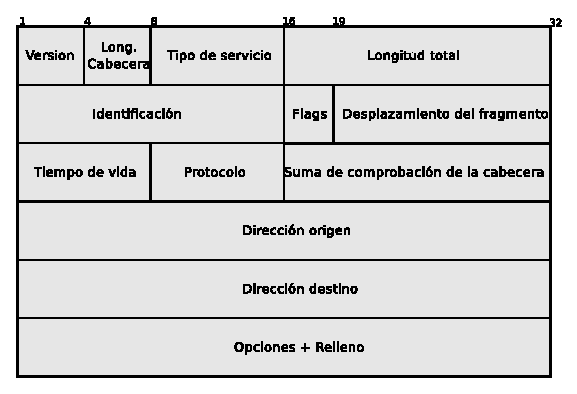
\includegraphics[width=1\textwidth]{2-sistema/graf/ip.eps}
  \caption{Formato de datagrama IP}
  \label{fig:ip}
\end{figure}

La PDU del protocolo IP se denomina \textit{datagrama IP} y se compone de los siguientes campos:
\begin{itemize}
	\item Versión: indica la versión del protocolo.
	\item Longitud de la cabecera: longitud de la cabecera expresada en palabras de 32 bits.
	\item Tipo de servicio: especifica los parámetros de fiabilidad, prioridad, retardo y rendimiento.
	\item Longitud total: longitud total del datagrama en Bytes.
	\item Identificador: un número de secuencia que, junto a la dirección origen y destino y el protocolo usuario, se utiliza para identificar de forma unívoca al datagrama.
	\item Flags: son 3 bits de los cuales solo 2 están definidos. El bit de \textit{no fragmentación} prohíbe la fragmentación cuando está puesto a 1. El bit de \textit{Más datos} se utiliza para fragmentación y reensamblado.
	\item Desplazamiento del fragmento: indica el lugar donde se sitúa el fragmento dentro del datagrama original, medido en unidades de 64 bits.
	\item Tiempo de vida: en cada enrutador se decrementa en 1 unidad. Tiene como fin evitar que un datagrama se quede dando vueltas para siempre en la red.
	\item Protocolo: especifica a que protocolo del nivel de transporte corresponde el datagrama.
	\item Suma de comprobación de la cabecera: Es el complemento a uno de la suma en complemento a uno de todas las palabras de 16 bits de la cabecera.
	\item Dirección origen: codificada para permitir una asignación variable de bits para especificar la red y el sistema final conectado a la red especificada.
	\item Dirección destino: igual que el campo anterior.
	\item Opciones: contiene las opciones solicitadas por el usuario que envía los datos.
	\item Relleno: se usa para asegurar que la cabecera del datagrama tenga una longitud múltiplo de 31 bits.
	\item Datos: debe tener una longitud múltiplo de 8 bits.
\end{itemize}

\subsubsection{Dirección IP}

Es un número de 32 bit que identifica un dispositivo dentro de una red que utilice el protocolo IP. Las direcciones IP se suelen representar por cuatro números decimales separados por puntos, que equivalen al valor de cada uno de los cuatro bytes que componen la dirección.

Como ocurre en la mayoría de las redes las direcciones IP tienen una estructura jerárquica. Una parte de la dirección corresponde a la red, y la otra al host dentro de la red. Cuando un dispositivo de enrutamiento recibe un datagrama por una de sus interfaces compara la parte de red de la dirección con las entradas contenidas en sus tablas (que normalmente sólo contienen direcciones de red, no de host) y envía el datagrama por la interfaz correspondiente.

Los bits que corresponden a la parte de red conforman lo que se denomina \textit{prefijo de red}.

Existen 3 maneras de representar un prefijo de red:

\begin{itemize}
	\item Binario con asterisco: por ejemplo, el prefijo 132.239 se denotaría 1000010011101111* (dado que 132 es en binario 10000100 y 239 es 11101111). El asterisco al final denota que los bits restantes pueden ser de cualquier valor.
	\item Notación A/L, donde A es una dirección IP y L es la longitud del prefijo. Siguiendo el ejemplo anterior, la notación sería 132.239.0.0/16.
	\item Notación máscara: pe utiliza una dirección de red y una máscara en vez de un prefijo explícito. De esta manera, volviendo al ejemplo anteriormente mencionado, éste puede expresarse como 132.239.0.0 con máscara 255.255.0.0
\end{itemize}
\end{comment}

La necesidad de procesar cada vez más paquetes de datos lleva a lo que se conoce como \textit{clasificación}. Ésta consiste en la categorización de paquetes en flujos de acuerdo a un conjunto de reglas determinadas. Se efectúa en base a campos en la cabecera del paquete, tales como la dirección IP de origen/destino, puerto de origen/destino, tipo de servicio (TOS), etc. En general, para una clasificación basada en N campos, se dice que esta es N-dimensional (o multidimensional). Cada regla \textbf{R} tiene \textbf{F} componentes y el $ f^{vo} $ componente de \textbf{R}, denotado como \textbf{R[f]} es una \textit{expresión de correspondencia de rango} en el $ f^{vo} $ campo del paquete. Si para todo \textit{f} $ \in $ [1, \textit{f}] el $ f^{vo} $ campo de la cabecera de un paquete \textbf{P} satisface la expresión de rango \textbf{R[f]}, \textbf{P} se corresponde con \textbf{R}.

Un caso particular de clasificación unidimensional es lo que se conoce como IP Lookup. Este sera abordado en el presente Proyecto Integrador.

\subsubsection{Dirección IP}

La dirección IP es un número de 32 bits que identifica un dispositivo dentro de una red que utiliza el protocolo IP. Las direcciones IP se suelen representar por cuatro números enteros separados por puntos, que equivalen al valor de cada uno de los cuatro bytes que componen la dirección.
La mayor parte de las redes IP contienen un grupo de direcciones IP jerárquicas. En general se entiende que una parte de la dirección corresponde a la red, y la otra al host dentro de la red. Cuando un dispositivo de enrutamiento recibe un datagrama por una de sus interfaces, compara la parte de red de la dirección con las entradas contenidas en sus tablas y envía el datagrama por la interfaz correspondiente.
Los bits que corresponden a la parte de red conforman lo que se denomina \textit{prefijo de red}.
Existen 3 maneras de representar un prefijo de red:

\begin{itemize}
	\item Binario con asterisco: por ejemplo, el prefijo 132.239 se denotaría 1000010011101111* (dado que 132 es en binario 10000100 y 239 es 11101111). El asterisco al final denota que los bits restantes pueden ser de cualquier valor.
	\item Notación A/L: donde A es una dirección IP y L es la longitud del prefijo. Siguiendo el ejemplo anterior, la notación sería 132.239.0.0/16.
	\item Notación máscara: se utiliza una dirección de red y una máscara en vez de un prefijo explícito. De esta manera, volviendo al ejemplo anteriormente mencionado, este puede expresarse como 132.239.0.0 con máscara 255.255.0.0
\end{itemize}

\subsubsection{IP Lookup}

El procedimiento que se lleva a cabo en un dispositivo de enrutamiento podría describirse de la siguiente manera:

Un paquete llega por una interfaz de entrada. Éste contiene una dirección IP determinada. El dispositivo consulta una tabla para encontrar una interfaz de salida para el paquete en cuestión. Dicha tabla contiene un conjunto de prefijos con sus correspondientes interfaces de salida. El paquete es correspondido con el prefijo más largo que esté contenido en la dirección de destino y luego es redirigido  a la correspondiente interfaz de salida. Esta tarea de determinar el enlace de salida es denominada Búsqueda de dirección (\textit{address lookup).}

En la figura~\ref{fig:prefijos} puede observarse una dirección IP como así también 3 prefijos de diferentes longitudes. Tanto éstos como la dirección están representados por sus bits. En el procedimiento de address lookup la interfaz seleccionada sería aquella asociada al prefijo más largo.

 \begin{figure}[h]
  \centering
	 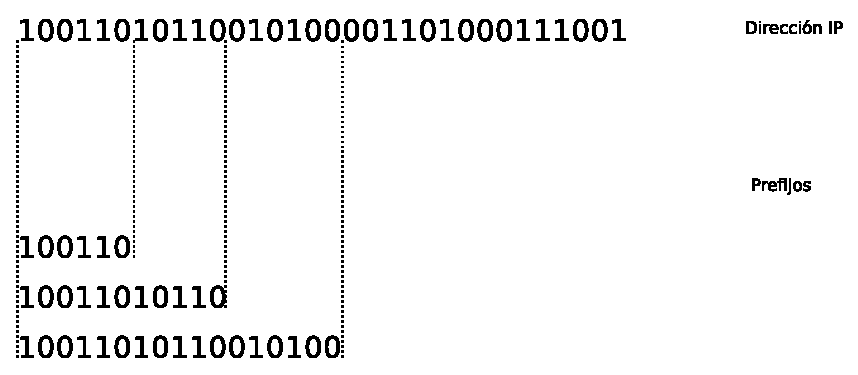
\includegraphics[width=0.7\textwidth]{1-introduccion/graf/prefijos.eps}
  \caption{Dirección IP y prefijos de diferente longitud}
  \label{fig:prefijos}
\end{figure}



\section{Objetivos}
\subsection{Objetivos Generales}
Teniendo en cuenta los problemas planteados, el objetivo general de este proyecto es estudiar los diversos algoritmos de clasificación de paquetes para poder encontrar sus limitaciones en la implementación tanto en software como en hardware. 
En particular, se considera una plataforma de lógica reconfigurable que permite integrar una arquitectura de hardware con software embebido.

\subsection{Objetivos Específicos}
Con el fin de cumplimentar los objetivos generales planteados, son necesarias las siguientes tareas:

    \begin{itemize}     

     	\item Diseñar un sistema embebido que realice la clasificación unidimensional de paquetes mediante una arquitectura mixta hardware-software.
	\item Implementar dicho sistema en hardware reconfigurable.
	\item Implementar al menos 2 algoritmos conocidos y analizar su rendimiento.
	\item Sugerir mejoras en la implementación de los mismos.

\end{itemize}


\section{Organización}

En el capítulo 2 se estudiará, a nivel funcional, una solución propuesta para este tipo de problemas. A continuación, en el capítulo 3, se presentará de manera detallada la arquitectura digital de los módulos que componen el sistema. En el capítulo 4 se describirá la metodología y los recursos utilizados para implementar este proyecto y en el capitulo 5 se presentan los resultados de esta implementación.





%\section{Distribucion Lineal}
